\chapter{Solución propuesta}
\label{chap:poc}

\if false

Para nuestro trabajo utilizaremos las librerías SEAL (como representante de la segunda generación) y THFE (como representante de la tercera).

Para ello comenzaremos con un estudio del funcionamiento de las librerías, de cuales son sus límites computacionales y pienso una operación que no sea "trivial" y a la vez sea computable por ambos.

La librería SEAL cuenta con varias operaciones aritméticas implementadas que pueden facilitarnos mucho el trabajo, así como la posibilidad de trabajar con matrices y número con coma flotante. La principal complicación con SEAL es calcular cómo se está desviando el cálculo para saber cuando parar o qué correcciones hacer. Además, las operaciones que puede hacer son relativamente limitadas (cuando se hacen, por ejemplo, productos, crece mucho el error). Si se ajustan los parámetros para realizar más operaciones o trabajar con números más grandes, se vuelve lentísima.

La librería TFHE ofrece una API de operaciones lógicas a nivel de bit. Aunque permitirá hacer cálculos más complejos sin añadir error al resultado, tendremos que implementar todas las operaciones a bajo nivel mediante puertas lógicas, siempre teniendo en cuenta que en ningún momento vamos a poder controlar el flujo de ejecución y nuestros algoritmos tienen que ser capaces de realizar los cálculos sin poder evaluar las variables (están cifradas), lo que hará que nuestras operaciones sean

Por lo tanto tenemos que encontrar un cálculo que sea realizable con pocas operaciones y números bajos para SEAL; y operaciones que sean implementables en un tiempo razonable con puertas lógicas para poder trabajar en TFHE.

Además, la operación que se realice con SEAL no puede contener más que sumas, restas y multiplicaciones (no existe la división).

He decicido hacer una regresión cuadrática de temperaturas de dos ciudades (esto lo haré con TFHE para poder hacer suma, resta, multiplicación y DIVISIÓN), que permitirá que un usuario en una fecha dada suba a SEAL su temperatura cifrada y averigue su localización.

Generaremos "el modelo" (la curva de regresión f(x)) con TFHE, porque para ello necesitaremos realizar operaciones muy costosas (elevando hasta la 4) y necesitamos dividir para hacer la media. Evaluaremos los datos introducidos por el usuario en SEAL (distancia entre f("x introducido por el usuario") y "y introducida por el usuario").
\fi

Para analizar las librerías he elaborado un sistema de posicionamiento anónimo en función de la temperatura y el mes del año.

En este sistema habrá tres actores: el cliente, el servidor de posicionamiento (programado con SEAL) y un tercer servidor (programado con TFHE) que generará el modelo para calcular la posición.

El cliente consultará su posición con el servidor de SEAL, que previamente habrá generado en el servidor de TFHE un modelo de posicionamiento basado en las temperaturas del último año en varias ubicaciones (ver \ref{fig:sistema_completo}).

\begin{figure}[h]
    \caption{Flujo de los datos cifrados\footnote{Diagrama generado con Piktochart \url{https://piktochart.com}}}
    \label{fig:sistema_completo}
    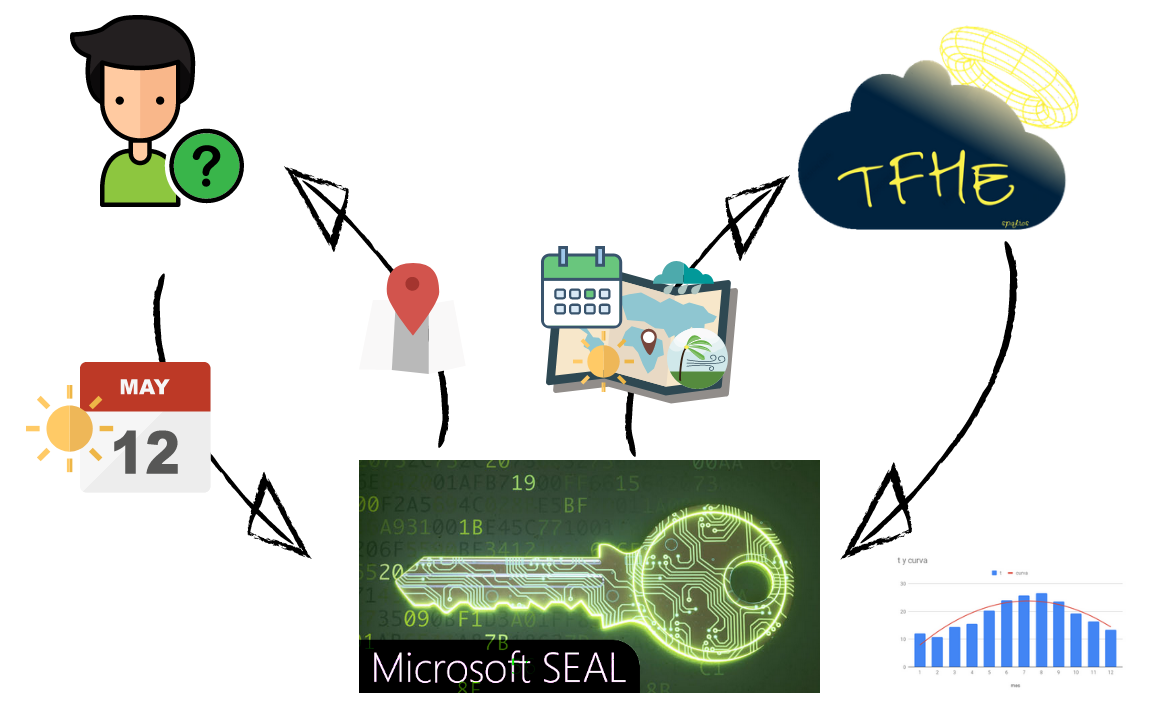
\includegraphics[width=\linewidth]{sistema_completo}
\end{figure}

Se han elegido tanto el sistema de ejemplo como las tecnologías específicas para cada uno de los actores en función de las capacidades y limitaciones de cada tecnología. Como resultado del proyecto se ha creado, además del análisis y el propio código del proyecto, una librería de operaciones matemáticas implementadas en TFHE (\cite{junquera_tfhe_2019}) con puertas lógicas, que es innovadora en tanto en cuanto no existe ningún código público que permita trabajar con TFHE a este nivel.

\section{Funcionamiento del sistema}

% TODO Gráficos de curvas de regresión con ejemplos

\subsection{Generación del modelo}

Para generar el modelo el cliente (en este caso, el servidor de posicionamiento con SEAL) y el servidor (el servidor con TFHE) seguirían el siguiente procedimiento:

1. El cliente genera un par de claves.

2. Cifra n pares de datos (en nuestro ejemplo el par sería (mes, temperatura)).

3. Sube los datos cifrados y su clave pública. El número de datos que se puede subir está limitado por el crecimiento del tamaño (en bits) de dichos datos al exponenciarlos para calcular la curva de regresión. Trabajaremos con los datos de 12 meses porque, como comentaremos más adelante\ref{chap:resultados}, aunque el orden máximo al que llegaríamos con estos datos es de 46 bits tendremos otras limitaciones a la hora de procesar los datos.

4. El servidor procesa los datos y devuelve cifrados los parámetros de la curva

5. El cliente los descifra y los almacena asociados a una posición geográfica

Finalmente, con los parámetros recibidos, el cliente obtendría una curva similar a \ref{fig:reg2_cg}.

\begin{figure}[h]
    \caption{Curva de Regresión Cuadrática con temperaturas de Cabo de Gata}
    \label{fig:reg2_cg}
    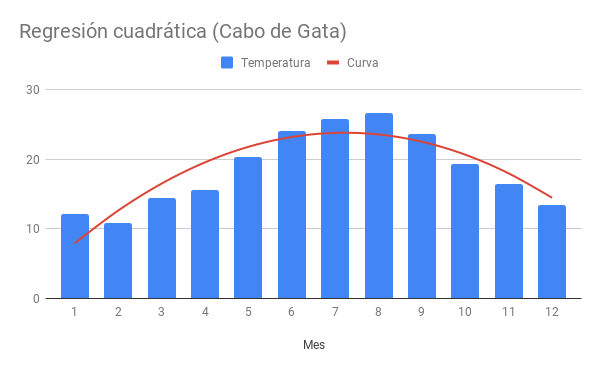
\includegraphics[]{reg2_cg}
\end{figure}

\subsection{Obtención de la posición}



\section{Implementación con TFHE}

Para generar la curva de regresión que utilizará el servidor de SEAL para ubicar al usuario, dicho servidor cifrará los datos de temperatura del último año en dos ubicaciones distintas y se las enviará al servidor TFHE. Este procesa los datos cifrados y calcula la regresión cuadrática codificada en tres parámetros $a, b, c$ que devolverá cifrados al servidor de SEAL.

$ DIAGRAMA PARA SUBIR DATOS DE SEAL A TFHE$

\subsection{Curva de regresión}

Esta curva $ y = f(x) $ está definida por tres parámetros ($a$, $b$ y $c$) de forma que:

\[ y = ax^2 + bx + c \]

Resultante de resolver el siguiente sistema de ecuaciones:

\begin{gather*}
    \begin{cases}
        \sum_{i=0}^n y_i = a*\sum_{i=0}^n x_i^2 + b*\sum_{i=0}^n x_i + n*c \\
        \sum_{i=0}^n y_i = a*\sum_{i=0}^n x_i^3 + b*\sum_{i=0}^n x_i^2 + c*\sum_{i=0}^n x_i \\
        \sum_{i=0}^n y_i = a*\sum_{i=0}^n x_i^4 + b*\sum_{i=0}^n x_i^3 + c*\sum_{i=0}^n x_i^2
    \end{cases}
\end{gather*}

Realizando las siguientes sustituciones:

\begin{align*}
    i &= \sum_{i=0}^n x_i & j &= \sum_{i=0}^n x_i^2 & k &= \sum_{i=0}^n x_i^3 & l &= \sum_{i=0}^n x_i^4 \\
    u &= \sum_{i=0}^n y_i & v &= \sum_{i=0}^n x_i * y_i & w &= \sum_{i=0}^n x_i^2 * y_i
\end{align*}

Obtendríamos un sistema lineal de ecuaciones solucionable mediante eliminación Gauss-Jordan:

\begin{gather*}
    \begin{cases}
        u = a*j + b*i + n*c \\
        v = a*k + b*j + c*i \\
        w = a*l + b*k + c*j
    \end{cases}
\end{gather*}

Además de la propia implementación con TFHE, se ha desarrollado un código de ejemplo en python mucho más legible \ref{regresion_cuadratica.py}.

TFHE sólo ofrece operadores lógicos, así que tenemos que escribir la operaciones aritméticas necesarias: suma, resta, multiplicación y división. Además tendremos que dar la posibilidad de trabajar con números reales, por lo que tendremos que determinar la codificación más apropiada. Para todo ello se ha desarrollado la librería \texttt{tfhe-math}

\subsection{tfhe-math}

$ OPERACIONES DE FUNCTIONS.h $

He hecho las siguientes operaciones aritméticas:

- Suma


\section{Implementación con SEAL}
